% Physikalisches Praktikum für Fortgeschritene
%  Universität Hamburg, Institut für Experimentalphysik
%  Versuch EXP18: "Top-Quark-Paare am LHC"

\def\ExperimentID{EXP18}
\def\ExperimentTitle{Top-Quark-Paare am LHC}

% ATTENTION:
%  DOCUMENT NEEDS TO BE COMPILED WITH EITHER XeLaTeX OR LuaLaTeX.
%  pdfLaTeX WON'T WORK DUE TO THE USE OF THE UNICODE-MATH PACKAGE
%  WHICH IS NEEDED FOR THE CORPORATE FONT OF UNIVERSITÄT HAMBURG.

% Type set using the memoir document class
%  Documentation to be found here: https://ctan.org/pkg/memoir
\documentclass[
    a4paper,
    12pt,
    oneside
]{memoir}

% Type set in "TheSans UHH" / LucasFonts -- Corporate typeface of Universität Hamburg
%  If you do not have access to this font yet, get it here, please:
%  https://www.kus.uni-hamburg.de/themen/oeffentlichkeitsarbeit/corporate-design/hausschrift.html
%  A system-wide font installation is not needed, you just have to place the
%  true-type files (.ttf) into the directory specified inside this variable:
\def\PathToTheSansUHH{./TheSansUHH/}
\IfFileExists{\PathToTheSansUHH/TheSansUHH-Regular2018.ttf}{
    \usepackage{unicode-math}
    \setmainfont[
        Path            = \PathToTheSansUHH,
        Extension       = .ttf,
        UprightFont     = *-Regular2018,
        UprightFeatures = {SmallCapsFont=*-SemiLightCaps2018},
        BoldFont        = *-Bold2018,
        BoldFeatures    = {SmallCapsFont=*-BoldCaps2018},
        ItalicFont      = *-RegularItalic2018,
        BoldItalicFont  = *-BoldItalic2018
    ]{TheSansUHH}
    \setmathfont{Fira Math}
    % Fira Math is a font similar to TheSansUHH but comes with dedicated
    %  math symbols which TheSansUHH does not have. In the following lines
    %  of code, we again replace the latin and greek math-mode alphanumeric
    %  letters of Fira Math with the ones of TheSansUHH for a consistent
    %  typeface. Note that this leads to some warnings which you may ignore.
    \setmathfont[
        range           = \mathup/{num,greek,Greek,latin,Latin},
        Path            = \PathToTheSansUHH,
        Extension       = .ttf
    ]{TheSansUHH-Regular2018}
    \setmathfont[
        range           = \mathit/{greek,Greek,latin,Latin},
        Path            = \PathToTheSansUHH,
        Extension       = .ttf
    ]{TheSansUHH-RegularItalic2018}
    \setmathfont[
        range           = \mathbfup/{num,greek,Greek,latin,Latin},
        Path            = \PathToTheSansUHH,
        Extension       = .ttf
    ]{TheSansUHH-Bold2018}
    \setmathfont[
        range           = \mathbfit/{greek,Greek,latin,Latin},
        Path            = \PathToTheSansUHH,
        Extension       = .ttf
    ]{TheSansUHH-BoldItalic2018}
}{%else
    % If you didn't put the TheSansUHH .ttf files into the specified directory,
    %  we will use the dedicated Palatino font (CMS standard!) as a substitute.
    \usepackage{newpxtext}
    \usepackage{newpxmath}
}
\usepackage[ngerman]{babel}

% Corporate design colors of Universität Hamburg
%  https://www.fid.uni-hamburg.de/corporate-manual.pdf
\usepackage{xcolor}
\definecolor{uhhred}{RGB}{226,0,26}
\definecolor{uhhblue}{RGB}{0,156,209} % for design elements
\definecolor{uhhblue-dark}{RGB}{0,133,179} % for blue text
\definecolor{uhhgray}{RGB}{59,81,91} % alternative to black text

% Page geometry
\settrims{0.0mm}{0.0mm}
\setlrmarginsandblock{2.5cm}{2.5cm}{*}
\setulmarginsandblock{2.5cm}{4.0cm}{*}
\checkandfixthelayout

% Layout of header and footer
\makepagestyle{uhh}
\makeoddhead{uhh}{\textcolor{uhhgray}{\bfseries\scshape Physikalisches Praktikum für Fortgeschrittene}}{}{\textcolor{uhhgray}{\bfseries\scshape \ExperimentID{}. \ExperimentTitle}}
\def\myhrulefill{\leavevmode\leaders\hrule height 0.382em\hfill\kern 0pt}
\makeoddfoot{uhh}{}{}{\hspace{0.618\textwidth}\textcolor{uhhblue}{\myhrulefill}\quad\textbf{\textcolor{uhhgray}{\Large Seite \thepage}}}
% Since this document is oneside, we don't need to set makeeven<foot|head>
\pagestyle{uhh} % activate the newly defined pagestyle
\copypagestyle{chapter}{uhh} % copy uhh style to first page of each chapter

% Layout of chapter headings
\chapterstyle{tandh}
%\renewcommand{\chapnumfont}{\bfseries\color{uhhred}\fontsize{48pt}{0pt}\selectfont}
%\renewcommand{\chaptitlefont}{\bfseries\color{black}\Huge}

% PDF metadata and PDF links
\usepackage[
    unicode, % required for XeTeX
    pdfencoding=auto,
    pdftitle={\ExperimentID{}. \ExperimentTitle},
    pdfsubject={Physikalisches Praktikum für Fortgeschrittene},
    linktoc=page,
    breaklinks,
    colorlinks,
    linkcolor=uhhblue-dark,
    citecolor=uhhred,
    urlcolor=uhhblue-dark
]{hyperref}

% More packages...
\usepackage{graphicx}
\graphicspath{{./images/}}

% Styling the markers in item list
\newcommand{\localtextbulletone}{\textcolor{uhhblue}{\raisebox{0.25ex}{\rule{0.382em}{0.382em}}}}
\renewcommand{\labelitemi}{\localtextbulletone}

% Some macros
\newcommand{\zB}{z.\,B.}
\newcommand{\pT}{$p_\text{T}$}
\renewcommand{\approx}{\text{ ≈ }}

\begin{document}

\begin{vplace} % vertically centered environment
\thispagestyle{empty}


\includegraphics[height=1.9cm]{images/UHH-Logo_2010_Farbe_CMYK}%
\hfill%

\includegraphics[height=3.1cm]{images/wortmarken}

\large
\centering
\newlength{\TitlePageSpacing}
\addtolength{\TitlePageSpacing}{.8cm}

\vspace{2\TitlePageSpacing}

\scshape
\textbf{Physikalisches Praktikum für Fortgeschrittene}\par\bigskip
 
\HUGE\normalfont
\textbf{\ExperimentID{}. \ExperimentTitle}\par

\vspace{.8\TitlePageSpacing}

\scshape

\large
\textbf{Versuchsbeschreibung} \\
Stand: \today{}\par\bigskip

\vspace{\TitlePageSpacing}
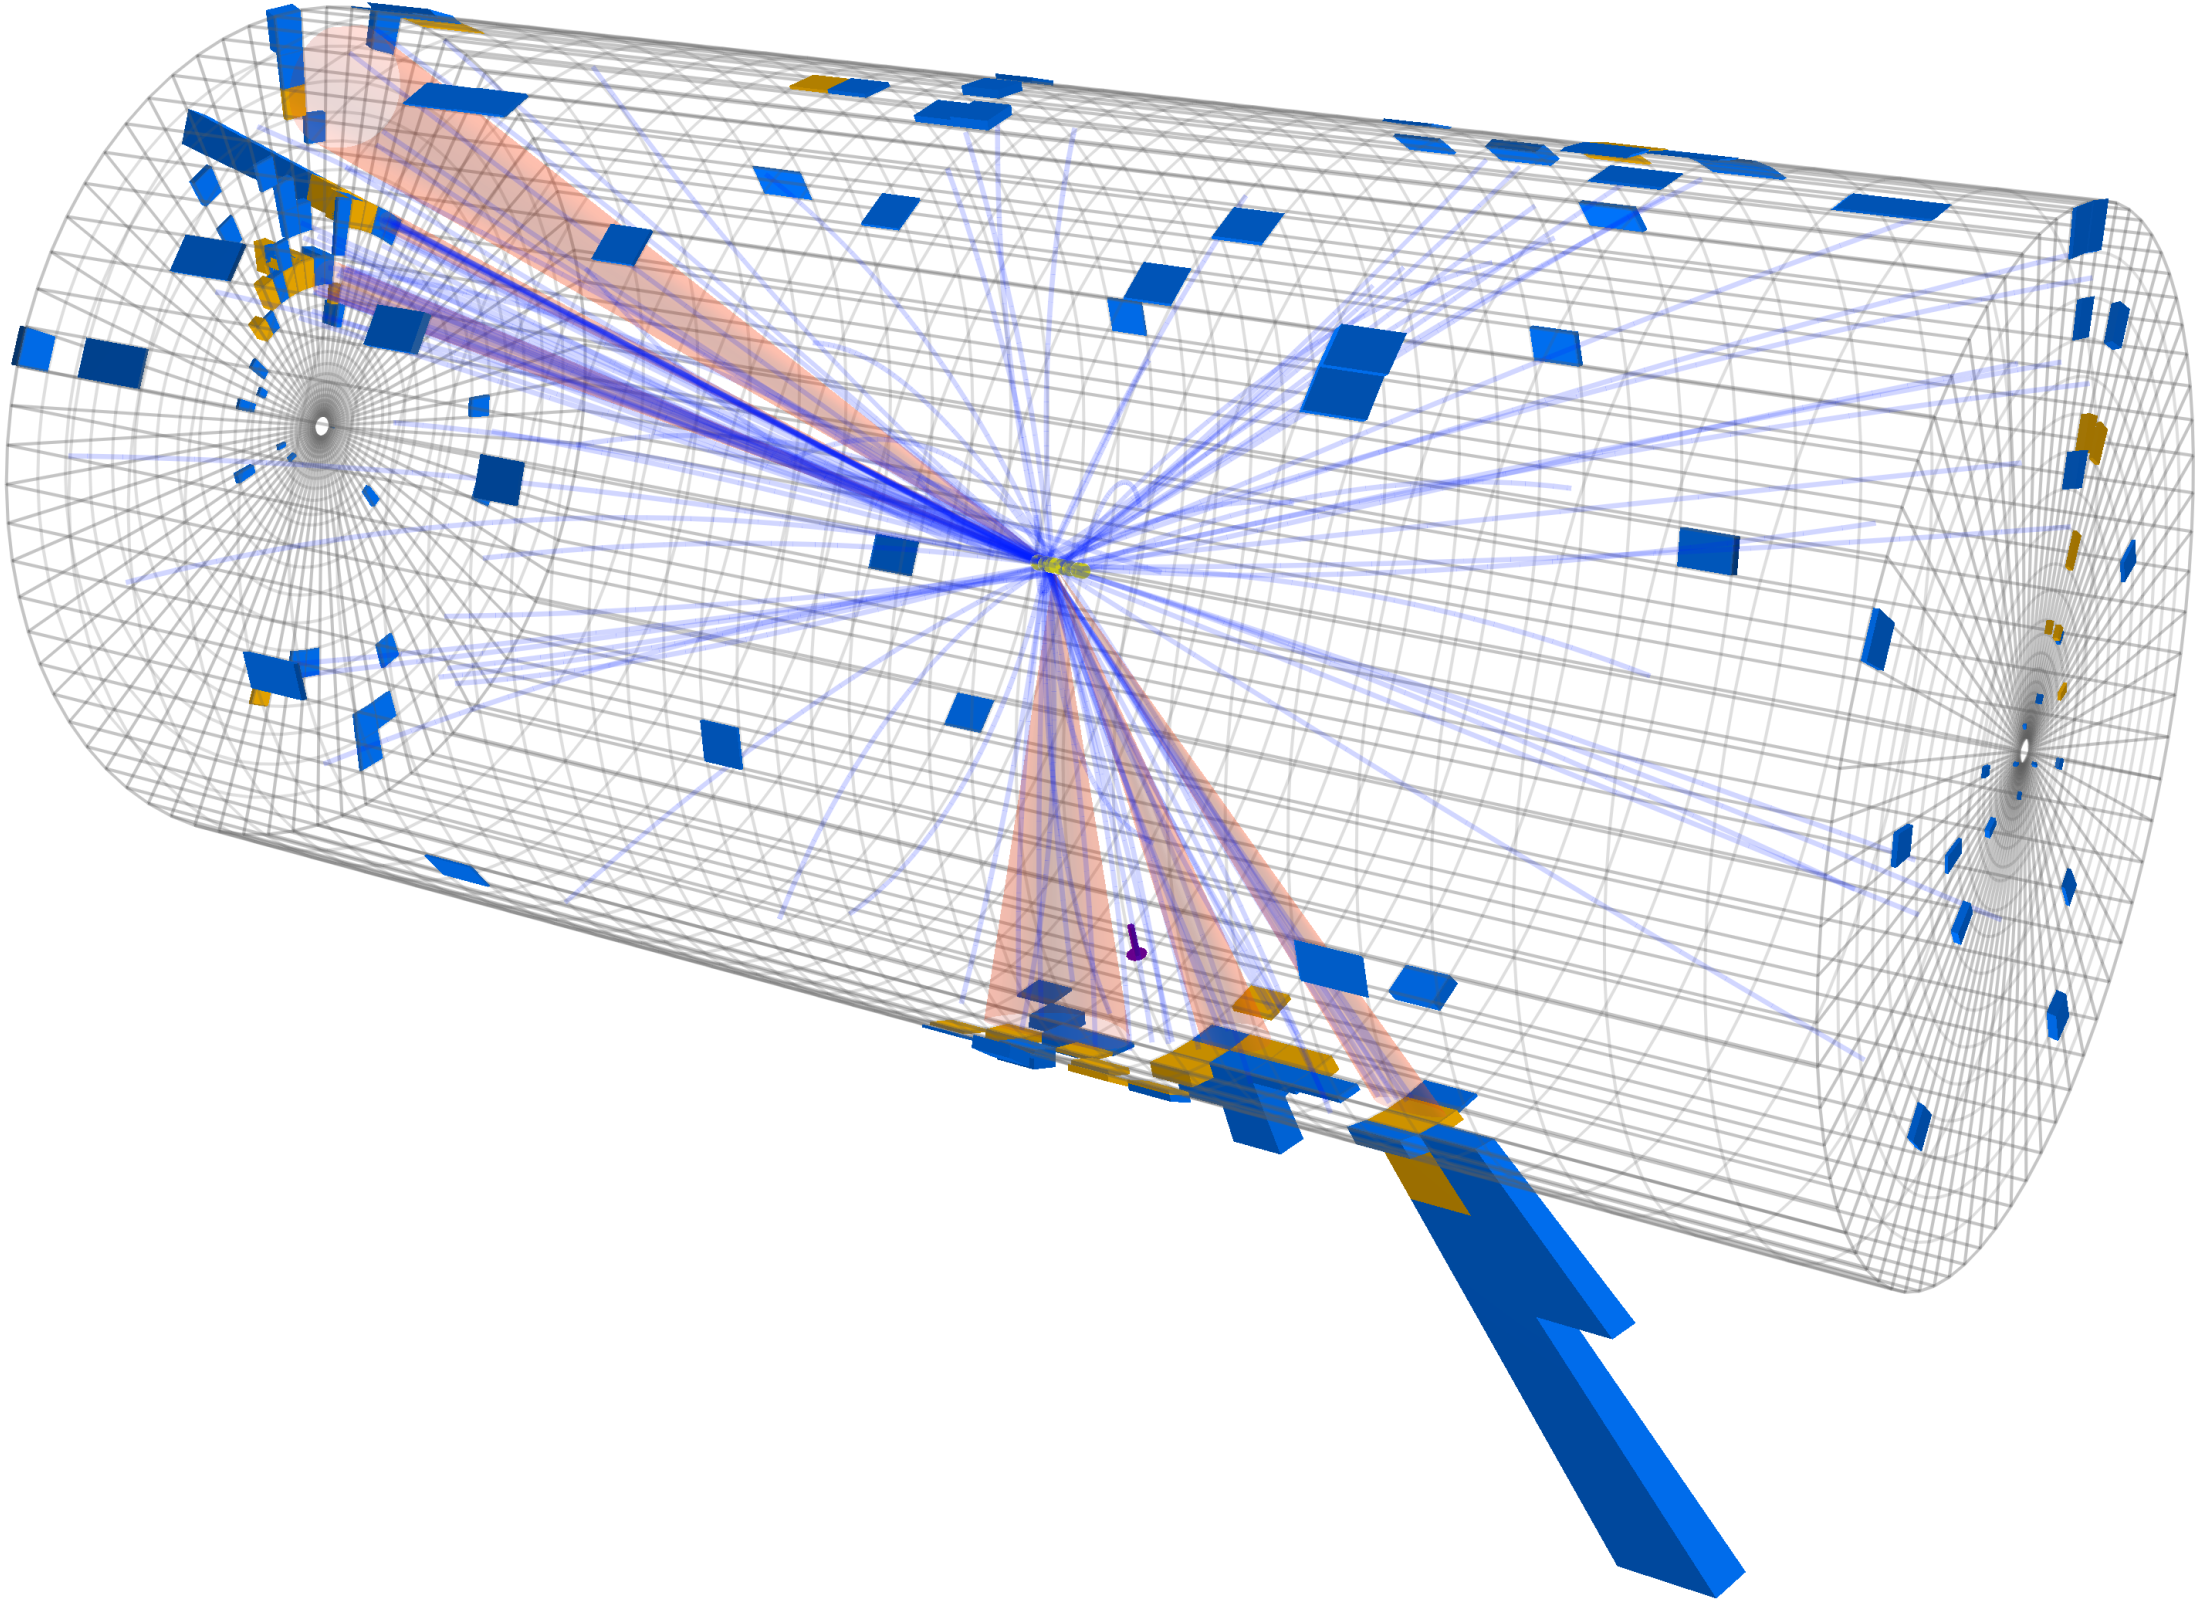
\includegraphics[height=6cm]{images/eventdisplay}
\vspace{\TitlePageSpacing}

\scshape

\textbf{Institut für Experimentalphysik} \\
Arbeitsgruppe Prof. Dr. Johannes Haller \\
Teilchenphysik \& Detektor-Entwicklung\par\bigskip

\textbf{Betreuer:} \\
Alexander Fröhlich \\
Christopher Matthies\par\bigskip

Basierend auf früheren Versionen von \\
A.~Reimers, J.~Multhaup und M.~Stöver

\end{vplace}

\clearpage
\OnehalfSpacing

\tableofcontents* % asterisk: no ToC self-reference
\addtocontents{toc}{~\hfill\textbf{Seite}\par}

\vfill
\noindent\tiny\textit{\textbf{Titelbild:} Simuliertes LHC-Kollisionsereignis, welches zur Paarerzeugung zweier Top-Quarks geführt hat. Eine solche Abbildung wird als "`event display"' bezeichnet. Gezeigt werden Signale im CMS-Detektor, ausgelöst durch die in alle Richtungen streuenden Endzustandsprodukte der Kollision. Die Top-Quarks selbst erreichen das Detektor-Material nicht, weil sie nahezu instantan wieder zerfallen, und müssen daher aus ihren Zerfallsprodukten rekonstruiert werden. Letzteres ist eine der Aufgaben dieses Praktikumsversuchs. -- Können Sie die Signaturen der Top-Quark-Zerfälle in diesem Ereignis per Auge identifizieren?}
\clearpage
\normalsize

\chapter{Einleitung}

\chapter{Theoretische Grundlagen}

%Dieses Kapitel stellt den wesentlichen theoretischen Hintergrund dar, welcher zum Verständnis dieses Praktikumsversuchs vonnöten ist. In Abschnitt \ref{sec:sm} wird das Standardmodell der Teilchenphysik, welches Ihnen aus der Vorlesung "`Physik 5"' geläufig sein sollte, zusammengefasst. Da sich dieser Versuch im Speziellen mit dem Top-Quark auseinandersetzt, bietet Ihnen Abschnitt \ref{sec:top} einen Überblick über dessen Eigenschaften und über die Top-Quark-Produktionsmechanismen am LHC.

\section{Das Standardmodell der Teilchenphysik}
\label{sec:sm}

Das Standardmodell (SM) der Elementarteilchenphysik bildet den theoretischen Rahmen zur Beschreibung der nach heutigem Kenntnisstand fundamentalen Bausteine der Materie und der Wechselwirkungen zwischen diesen. Das SM ist eine Quantenfeldtheorie, deren Anfänge bis in die 1940er Jahre zurückdatieren und welche in den darauffolgenden Jahrzehnten aus verschiedenen Motivationen heraus mehrfach erweitert worden ist\footnote{Im Speziellen bezieht sich diese Aussage auf die Begründung der Quantenelektrodynamik (QED) durch Richard Feynman \textit{et al.} und die spätere Anwendung der gleichen theoretischen Konzepte auf die starke und schwache Kernkraft in den 1970er Jahren.}. Einerseits waren die Weiterentwicklungen der Theorie begründet durch neue Beobachtungen, die von der experimentellen Teilchenphysik gemacht worden sind, andererseits sind auch viele Fälle zu verzeichnen, in denen die Theorie dem Experiment zuvorgekommen ist. Das heutzutage prominenteste Beispiel für die Vorhersagekraft des SM ist der Nachweis der Existenz des Higgs-Bosons am LHC (vgl. Physik-Nobelpreis 2013).

Trotz des großen Erfolgs des SM ist es nicht in der Lage, sämtliche physikalischen Phänomene zu erklären, die in der Natur beobachtet werden können. So wird beispielsweise Gravitation bisher nicht durch eine Quantenfeldtheorie beschrieben, die mit dem SM vereinigt werden könnte. Des Weiteren beinhaltet das SM weder Teilchen, die als Kandidaten für dunkle Materie infrage kämen, noch liefert es irgendeine Erklärung für die mutmaßliche Existenz dunkler Energie. Diese und weitere Umstände veranlassen Teilchenphysiker dazu, die momentan etablierte Theorie auf die Probe zu stellen (Präzisionstests des SM) und potentielle Erweiterungen des SM experimentell zu überprüfen (Suche nach neuen Teilchen, Wechselwirkungen und anderen Effekten\footnote{Zusammenfassende Oberbegriffe: "`Neue Physik"' bzw. "`Physics \textbf{b}eyond the \textbf{S}tandard \textbf{M}odel"' (BSM).}).

\section{Physik von Proton-Proton-Kollisionen}
\label{sec:pp}

\section{Physik des Top-Quarks}
\label{sec:top}

\chapter{Der CMS-Detektor am LHC}


\begin{appendices}
\chapter{Fragenkatalog zur Vorbereitung}

\begin{itemize}
\item Warum wird generell eine sehr große Anzahl an Kollisionsereignissen benötigt, um aussagekräftige Teilchenphysik-Studien durchzuführen? -- Würde es beispielsweise für die Bestimmung der Top-Quark-Masse ausreichen, auf ein einzelnes Ereignis zu warten, das ein Top-Quark enthielte, wonach man den LHC abschalten und Feierabend machen könnte? Wenn nicht: Warum wird eine große Anzahl an Ereignissen benötigt, in denen Top-Quarks produziert werden?
\item Warum wird am LHC vornehmlich auf transversale Größen rekonstruierter Objekte zurückgegriffen (\zB{} auf den transversalen Impuls, \pT{})? 
\end{itemize}

\end{appendices}

\end{document}